% #############################################################################
% This is Chapter 4
% !TEX root = ../main.tex
% #############################################################################
% Change the Name of the Chapter i the following line
\fancychapter{Architecture}
\cleardoublepage
% The following line allows to ref this chapter
\label{chap:arch}

The fundamental objective of this work is to develop a portable device,  which enables entities to establish secure channels of communication.
A solution was developed on a portable HSM, which secures communications between users, stores the owner's sensitive data, such as keys, and performs all services critical to its security. This is an easy process for the owner, who does not need to concern himself with any setup or management, the system is accessible and ready to use when received.
This chapter presents an overview of the developed system, its services, the protocol used for communications and use cases, unconstrained by a specific physical device.

% -----------------------------------------------------
% -----------------------------------------------------
\section{Overview}\label{chap:arch:overview}

%% COMPONENTS INTRODUCTION %%
The system, pictured in Figure~\ref{fig:overview}, is composed of two main components: the physical device, responsible for all operations, and the application on the user's computer, which provides a straightforward interface to users.

\begin{figure}[h]
    \centering
    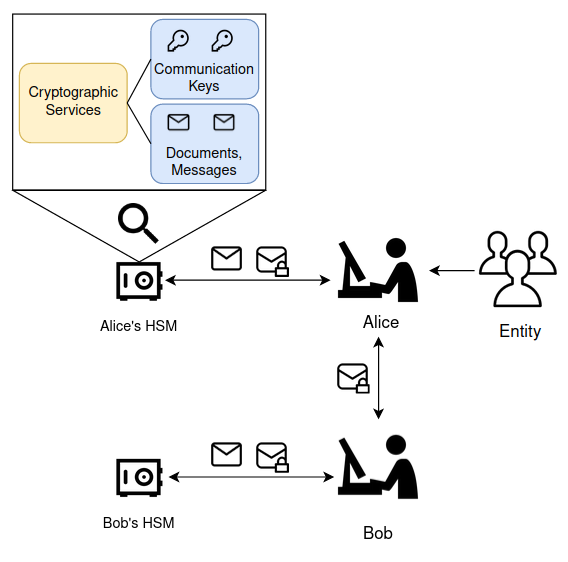
\includegraphics[width=0.75\textwidth]{./Images/overview2.png}
    \caption{System Overview}
    \label{fig:overview}
\end{figure}

%% SYSTEM OVERVIEW %%
The user's computer running the software is connected to the device, through a physical connection, used to send and receive data and commands.
Using these tools, the user can request the device to perform the desired services.
These services are implemented inside the device, which stores and manages keys, as well as other data.
If the device is misplaced or stolen, the stored keys and documents are not at risk of being extracted. The developed software and physical tamper measures ensure it.
Upon receiving their device, each user is only required to connect it to their computer using the appropriate cable. The system is ready to use, through the provided interface software, which should be used in the user's personal computer.

% -----------------------------------------------------
% -----------------------------------------------------
\section{Services}\label{chap:arch:services}

%% INTRODUCTION %%
This section describes each system service and all its relevant information. 
Firstly, it presents the authentication, then the secure data exchange service, qualified digital signatures and services to establish new communication endpoints.

% -----------------------------------------------------
\subsection{Authentication}\label{chap:arch:services:auth}

Each entity will have its own device, which can be connected to a computer. To access the device's services, all users need to be authenticated to the device, through a PIN, which is securely stored inside the device. There is only a single PIN, used to authenticate the entity to their device.
Each entity can supply this PIN to users, which will use the device on behalf of the entity.
After the user sends the correct PIN and is authenticated, the PIN can be changed.

% -----------------------------------------------------
\subsection{Secure Data Exchange}\label{chap:arch:services:data-exchange}

As previously introduced, the main goal of this solution is to secure communications between multiple entities, with identical devices.
Herein defined is the secure data exchange service, responsible for securing communications between entities. 
Communications are secured by providing three services: confidentiality, integrity and authentication. This allows communicating entities to ascertain the origin of messages and prevent unauthorized entities from reading and modifying them.
To grant these services, communicating entities must agree on a symmetric key. This key will be stored in the devices of both entities, and is never exposed outside the device. In order for entities to agree on a key, the system provides services which will be discussed further ahead. In order to describe the secure data exchange service, we will assume a symmetric key has already been agreed between both entities.
% This system provides services for key agreement between entities, which will be discussed further ahead.

As discussed in the previous chapter, and depicted in Figure \ref{fig:overview}, Alice's computer will communicate with her HSM, in order to secure data, to be sent to Bob. For this, there needs to be a communications protocol between the computer and HSM, to define what data is sent, in what order and by who. To secure a piece of data sent by Alice, the device needs to receive the data, and return the data encrypted and authenticated with an internal key, previously agreed by Bob and Alice.
Thus, the communication protocol, between the device and computer application, is illustrated in Figure~\ref{fig:protocol:data-exchange}.

\begin{figure}[h!]
	\centering
	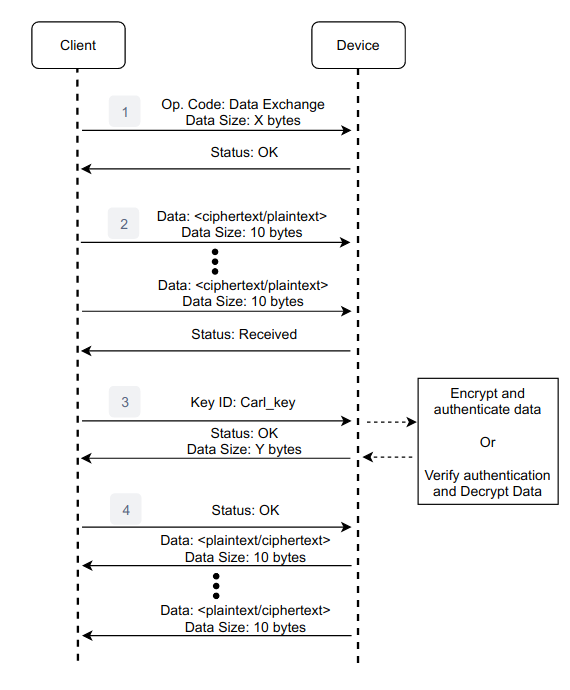
\includegraphics[width=0.60\textwidth]{./Images/data-exchange.png}
	\caption{Communication protocol for data ciphering and authentication in the HSM with internal keys}
	\label{fig:protocol:data-exchange}
\end{figure}

Since the system is designed to have multiple services, and be able to store multiple keys, there needs to be a mechanism to identify the different services and keys.
Services will be identified through an operation code, with an unique value for each service. Similarly, keys will be identified through an ID with an unique value for each key. Alice must know the ID for every key and to what entity it was agreed with. The ID is stored in the device along with the corresponding key.

Thus, if Alice wants to secure data, the computer must first send a message composed of a code, identifying the secure data exchange service, and the key ID, to identify the symmetric key which will be used to secure data.
Upon receiving the message, the device will check internally if the user is authenticated and if both the operation code corresponds with an existing service and if the key with the corresponding ID exists.
Subsequently, the corresponding success or failure status is returned by the device.

After a successful exchange, the data can be sent to the device. Before the data is received, the device must know the size of the data which it will receive from the computer. % Thus, 2 bytes containing the data size are sent first.
After the data is processed in the device, its output is sent back to Alice, which can be securely sent to another entity, with the same symmetric key in their device.
If Bob wants to obtain the plaintext of the data sent by Alice, the same communication process is used. Bob sends the correct operation code and key ID, receives a success status response, then sends the secured data from Alice, and waits for the plaintext response from the device.

To produce the secure data, the plaintext must be encrypted and authenticated to provide the three necessary cryptography services: confidentiality, authentication and integrity.
On the other hand, there must also be a process to authenticate and decrypt the data, in order to retrieve the plaintext. Therefore, a protocol for encryption and encryption with authentication is needed.

As presented in Section \ref{chap:background:crypto}, symmetric encryption schemes provide confidentiality to data, while MAC algorithms provide authentication. AEAD schemes, which authenticate and encrypt messages, such as AES-GCM, may be more efficient and are less likely to be misused, compared to combining separate encryption and authentication schemes.
Unfortunately, devices such as the SmartFusion2 SoC, do not provide AEAD schemes. These boards usually provide separate encryption and authentication algorithms.
Thus, to mitigate this problem, the proposed solution combines an encryption and authentication scheme, in order to provide the necessary cryptography services.
Both algorithms can be combined in different orders. Studies recommend combining a secure encryption and secure MAC, with the encrypt-then-MAC method~\cite{encryptmacorder}. This method encrypts the plaintext first, then generates the MAC from the generated ciphertext.

From this information, the proposed encryption protocol is pictured in Equation \ref{eq:encrypt-mac}. First, the plaintext data is encrypted with an internal symmetric key and a randomly generated IV. Next, a MAC is generated from the concatenated IV and ciphertext.
If the IV can be modified by an attacker, the original plaintext cannot be fully recoverable. Therefore, it is important that the MAC is generated from both the ciphertext and IV, this way the receiver can detect if either information was altered.
The output data is the concatenation of the IV, ciphertext and MAC.
\begin{equation}
	\label{eq:encrypt-mac}
	E_{key}\{Data, IV\}, MAC_{key}\{IV+E_{key}\{Data, IV\}\}
\end{equation}

The decryption protocol is pictured in Equation \ref{eq:decrypt-mac}. The protocol follows the same process as the previous protocol, but in reverse order. First, a new MAC is generated from the received IV and ciphertext. Then, the computed and received MACs are compared. If identical, the receiver can be sure of the data's origin and integrity. The ciphertext is decrypted with the same internal symmetric key used for encryption and the received IV, to obtain the plaintext.

\begin{equation}
	\label{eq:decrypt-mac}
	(MAC_{key}\{IV+Ciphertext\} == MAC) => E_{key}\{Ciphertext, IV\} => Data
\end{equation}

% ----------------------------------
\subsection{Qualified Digital Signatures}\label{chap:arch:services:signatures}

Digital signatures provide non-repudiation to a piece of data. This prevents an entity from denying the authorship of a message. Qualified signatures are a special type of signatures where the private keys, which generated them, are stored inside a device, such as a HSM, and are never exposed to the outside.
Therefore, the signature must be generated inside the HSM, and the device should support an algorithm for the generation of signatures.
The private key, which will generate signatures, identifies the entity and is stored inside the device. In order for the device to be ready for the generation of signatures, a private and public key pair must be randomly generated in the device, or imported from the outside if the device does not support this. This must be done before the device is delivered to entities.
%the key must be randomly generated and subsequently stored in the device, before it is delivered to entities.

As with the previous service, a communications protocol between the user and device must be defined. The device must receive the data, from which it will generate the signature, while the user will receive the generated signature.
The devised communication protocol is presented in Figure~\ref{fig:protocol:signature-generate}.

\begin{figure}[h!]
	\centering
	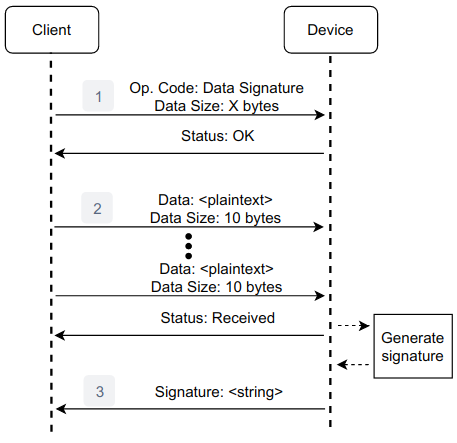
\includegraphics[width=0.55\textwidth]{./Images/signature-generate.png}
	\caption{Communication protocol for generating digital signatures using internal HSM asymmetric key pair}
	\label{fig:protocol:signature-generate}
\end{figure}

In order to identify the service, the user will send the corresponding operation code, along with the data to be signed.
Upon reception of the data, the device checks if the user is authenticated and subsequently generates the qualified signature, using its internal private key.
Afterwards, the device responds with the generated signature. 
Other entities can validate the signature using the author's public key. Only the entity, in possession of their device with its private key, could have generated the signature.

As discussed previously, public key cryptography is slow. Therefore, a digital signature is generated by first computing a hash of the message, then signing the hash with the private key, as shown in Equation \ref{eq:signature-generate}. In general, generating a signature from a hash is faster, since it has a small fixed size, while the signed data can be of any size.

\begin{equation}
	\label{eq:signature-generate}
	Sign_{K}\{Hash\{Data\}\}
\end{equation}

% To verify a signatures, the user sends the operation code, signature length and generated signature, as well as the data length and data from which the signature was generated. The last piece of information sent is the public key of the device, where the signature was generated.
% After verifying the signature, the device responds with the operation status.
% The data is verified using the same hash function, ECDSA algorithm, and the signers' public key, as detailed in \ref{eq:signature-verify}.

% \begin{equation}
%         \label{eq:signature-verify}
%         \{Signature\} == Verify_{K_{-1}}\{Hash\{Data\}\}
% \end{equation}

% -----------------------------------------------------
\subsection{Establishing New Communication Endpoints}\label{chap:arch:services:new-comms}

The system provides the flexibility to establish secure communications with new entities, with identical devices.
To achieve this, entities must agree on a new symmetric key, which can be subsequently used with the secure data exchange service, presented in Section \ref{chap:arch:services:data-exchange}, to secure communications between them.
All new keys are stored in the device's secure storage, along with its unique ID.
Two different mechanisms to generate and agree on new symmetric keys are presented next. The first uses public key cryptography and the second uses symmetric key cryptography.

% -----------------------------------------------------
\subsubsection{Key Generation}\label{chap:arch:services:new-comms:ecdh}

As introduced in Section \ref{chap:background:crypto:ecdh}, two entities can agree on a symmetric key, using public key cryptography.
Both entities must have a private and public key pair, and share both public keys with the other entity. Only the private key must remain a secret, the public key can be shared. Then, both entities can generate the same key, using their private key and the peer's public key.

Just like previous services, there needs to be a communication protocol to trade the necessary information, and generate the key. The device must receive the peer's public key and return its own public key. After this trade, the key is generated and stored in the device. Following these guidelines, the protocol to generate a shared symmetric key with another entity, using asymmetric cryptography, is detailed in Figure~\ref{fig:protocol:ecdh}.
\begin{figure}[h!]
	\centering
	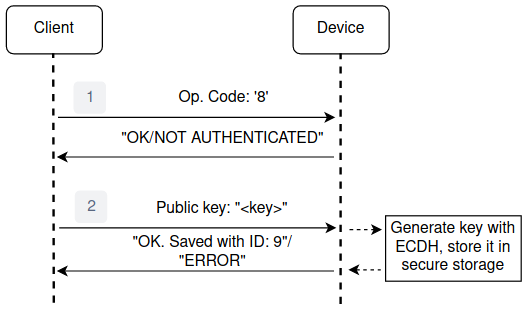
\includegraphics[width=0.60\textwidth]{./Images/ecdh.png}
	\caption{Communication protocol to generate a symmetric key with another entity, using an internal private key}
	\label{fig:protocol:ecdh}
\end{figure}

The protocol starts with the user sending the operation code, signaling the device it wants to generate a symmetric key. The device responds with its public key, which needs to be shared with the other entity. After the user receives the peer's public key, it forwards this key to the device, and waits for a response. If successful, the device internally generated the symmetric key, which is now stored in its secure storage. The device also returns the new key ID to the user, so the entity can keep track of the ID which it needs to use to securely communicate with the other entity.
The internal key generation process only needs the internal private key and the received public key.

As mentioned, both entities must share their device's public key with the other entity. They must do it in a way, so that they can be sure the received public key is from the actual entity they wish to communicate with, and not an impersonator. This is usually achieved by a PKI, which is a trusted third party which stores, validates and distributes public keys. 

Instead of entities sharing public keys using an untrustworthy communication service, with no validation of the traded public keys, a PKI inspired system can be used. 
In this system, keys are exchanged using an intermediary, which is a special entity, trusted by both sides. Both entities should have previously agreed keys with the special entity, so they can securely send their public key. Thus, the special entity is responsible for distributing the public keys. Entities can trust the received keys belong to the correct entity.

% -----------------------------------------------------
\subsubsection{Import Keys}\label{chap:arch:services:new-comms:import}

The key importation service provides a mechanism to share and import keys to the entities' devices using symmetric key cryptography. This alternative provides flexibility to the system.
Users are not constrained to key sharing using public key cryptography. This service also provides a mechanism to solve another problem. If symmetric keys are used incorrectly or for too long, attackers can collect enough data to potentially break the security of keys. This can be mitigated by this service, since it allows updating the existing keys, to avoid its overuse.

In order to import the keys, the device receives an encrypted and authenticated list of keys, decrypts them with the secure data exchange service used for secure communications and overwrites the existing internal keys in the device.
The communication protocol for this service is depicted in Figure \ref{fig:protocol:import-keys}.
\begin{figure}[h!]
	\centering
	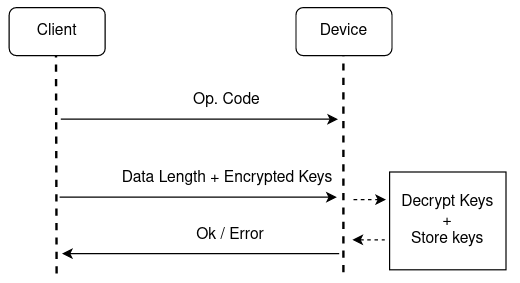
\includegraphics[width=0.60\textwidth]{./Images/import-keys.png}
	\caption{Communication protocol to import encrypted and authenticated symmetric keys, and store them in the HSM}
	\label{fig:protocol:import-keys}
\end{figure}

The operation code, sent by the user, signals the device it will subsequently receive a list of keys. Upon receiving the keys, the device authenticates and decrypts the keys using an internal key.
Each key on the list is accompanied by 1 byte for its size and 1 byte for its ID.

As mentioned, the keys are received encrypted and authenticated. This must have been previously processed by another special entity, using the secure data exchange service.
The entity importing the keys into their device, must have a symmetric key in their device, to communicate with the special entity. This entity called "control station", was introduced in the previous chapter.
The sole purpose of the entity is to act as a trusted third party, which distributes keys to the entities, through the secure data exchange service.
Each system must be delivered to entities with an internal symmetric key for communications with the control station. Thus, entities can communicate with the control station to request keys with no setup or key agreement necessary.

Whenever an entity wishes to communicate with others, they can send a list of entities they intend to communicate with to the station, secured with the data exchange service. The control station subsequently supplies the user with the list of keys, to be imported in their device.
For example, if Alice wants to communicate with Bob, Alice can request the key from the control station. Then, the control station generates the key and sends it to both Bob and Alice, encrypted and authenticated with different predefined keys for both.
Alice and Bob use this service to import the key into their devices, and can subsequently begin secure communications between each other.

% The ciphertext and randomly generated IV are stored in memory. Both are authenticated by generating a MAC and storing it in secure storage.
% In order to fetch a stored key, a MAC is generated from the ciphertext and IV in memory, and compared to the MAC in secure storage. If identical, the keys can be decrypted and a specific key identified through its ID.

% The device can also import a new set of keys, provided by the control station.
% This way, already established channels of communication can be updated on a regular time schedule.
% When a user wants to communicate with a new entity, the system provides two convenient solutions.
% Both options allow establishing connections with new entities when needed, by way of a trusted third party: a control station.
% The user can securely contact the control station at any time to request the public key of the other entity, through the secure data exchange service, equivalent to communicating with any other entity. The control station effectively acts as a PKI.
% Then, the user sends the information through the computer application to the device. The new key is generated in the device and made available right away. Then data can be exchanged with the new entity, which must also request the control station for the analogous entity's public key.

% The system can also be setup with a regular communication update schedule. It grants the flexibility of key revocation when needed, data exchange with new entities, as well as updating symmetric keys, with no additional complexity to the user, to always safeguard the security of communications.
% Each month an entity can hand over a list of the entities it wishes to communicate with to the control station, which will accordingly yield the corresponding key set.
% Each entity only needs to forward the list to the device, and the new keys are immediately stored and ready to be used.
% Users can resume communications, the same way as before with minimal interruption, with the requested entities.
% The protocols for both services are detailed next: symmetric key generation and importation of keys.

% -----------------------------------------------------
\section{Summary}\label{chap:arch:summary}

This chapter presented the system's functionalities, algorithms and communications protocols, between a secure and portable device, and the user's computer.
The system grants confidentiality and authentication to communications between any number of users, as soon as they receive the device, without overloading the users with convoluted tasks or responsibilities.
It provides entities with the flexibility to manage which entities they wish to communicate with by themselves, or by offloading the management responsibility to a trusted control station.
